\section{Menu główne (Zofia Sosińska)}\label{chap:menu_main_impl}
Przed startem właściwej gry, użytkownikowi ukazuje się menu główne. Pełni ono funkcję reprezentatywną, więc ważne jest, aby współgrało ono z głównym programem.
Styl okna jest prosty i surowy, stawiając na skalę szarości przy doborze kolorów. Nawiązuje on do stylu interfejsu użytkownika występującego 
w trakcie rozgrywki. Sprawia to, że gracz jeszcze przed zanurzeniem się w świat gry, ma jego przedsmak.

Zgodnie z projektem menu główne udostępnia trzy kluczowe funkcjonalności:
\begin{itemize}
    \item rozpoczęcie nowej gry,
    \item wczytanie zapisanej gry,
    \item wyjście z programu.
\end{itemize}

Przycisk nowej gry przenosi użytkownika do momentu startowego rozgrywki. Progres gry jest równy zeru, a wszystkie zadania dopiero czekają na wykonanie.

Po kliknięciu przycisku odczytu pojawia się lista zapisów, które w przeszłości użytkownik zdecydował się permanentnie przechować w pamięci urządzenia, na którym
włączony został program. Użytkownik może ją przeglądać ruszając suwakiem po prawej stronie. Po wybraniu jednej z opcji zostaje przeniesiony 
do świata gry o stanie takim, jaki został wczytany z pliku.

Ostatni przycisk udostępnia funkcjonalność wyjścia z gry. Po jego naciśnięciu użytkownik całkowicie wyłącza program.
\begin{figure}[htbp]
    \centering
    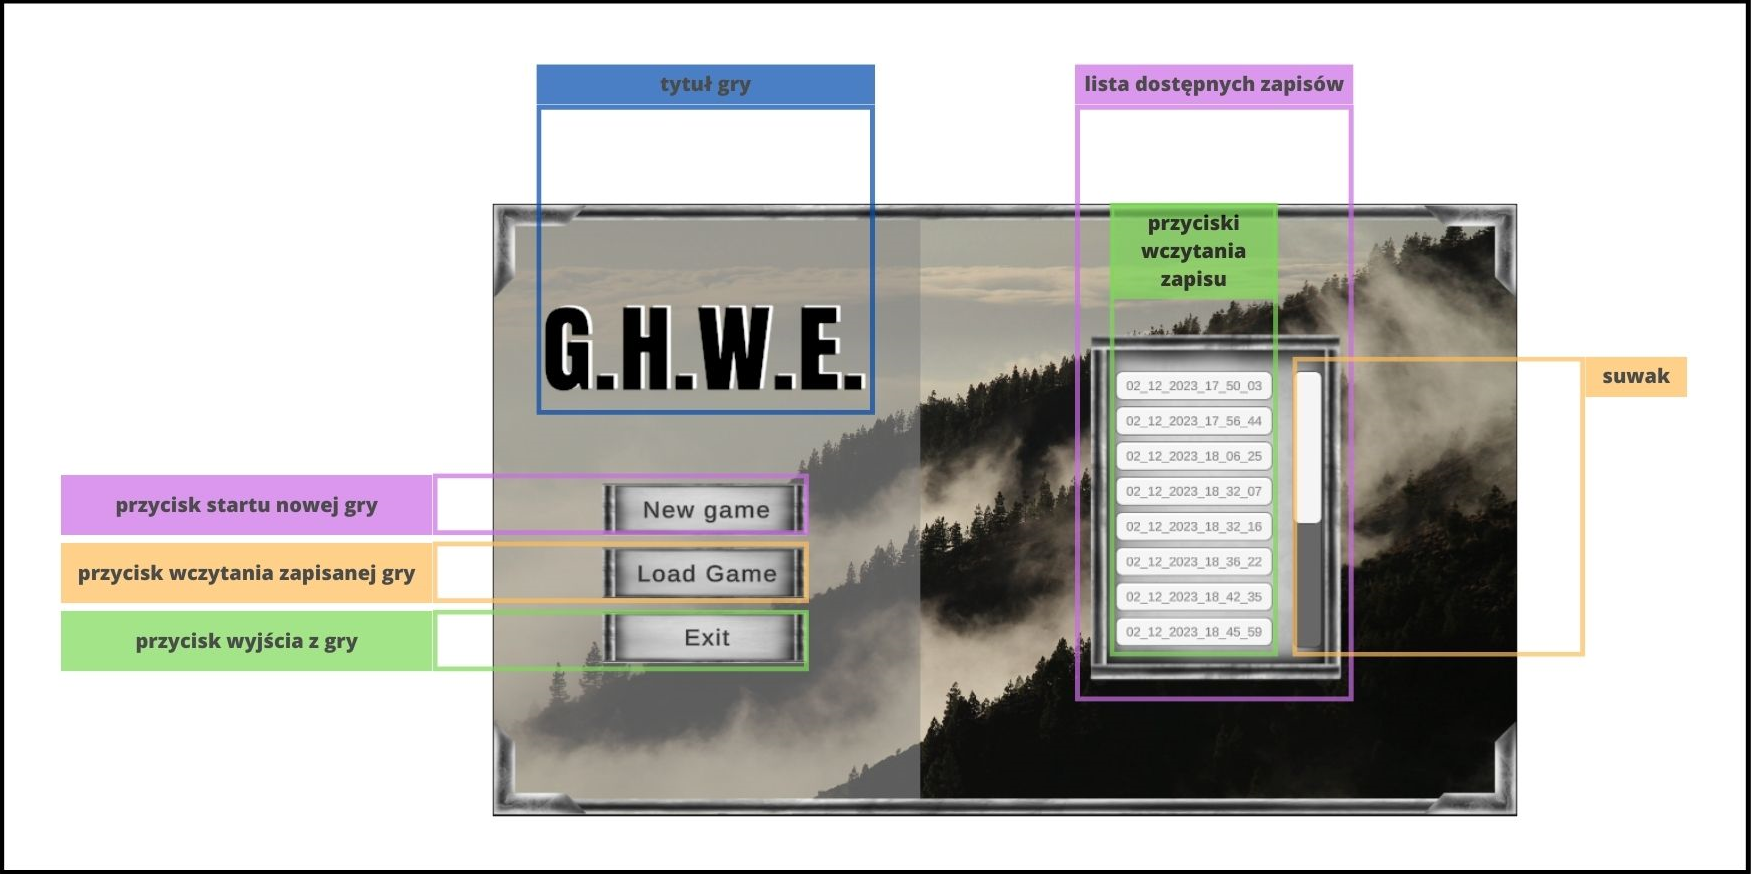
\includegraphics[width=0.9\textwidth]{images/ui/main_menu.png}
    \caption{Implementacja menu głównego.
    }\label{fig:compass}
\end{figure}
